\documentclass{beamer}

\usetheme{Boadilla}

%\includeonlyframes{current}

\usepackage{times}
\usefonttheme{structurebold}
\usepackage{listings}
\usepackage{ragged2e}

\usepackage{pgf}
\usepackage{tikz}
\usepackage{alltt}
\usepackage[normalem]{ulem}
\usetikzlibrary{arrows}
\usetikzlibrary{automata}
\usetikzlibrary{shapes}
\usepackage{amsmath,amssymb}
\usepackage{rotating}
\usepackage{ulem}
\usepackage{listings}
\usepackage{enumerate}
\usepackage{tikz}
\tikzset{
  every overlay node/.style={
    draw=black,fill=white,rounded corners,anchor=north west,
  },
}
\def\tikzoverlay{%
   \tikz[baseline,overlay]\node[every overlay node]
}%

%\setbeamercovered{dynamic}
\setbeamertemplate{footline}[page number]{}
\setbeamertemplate{navigation symbols}{}
\usefonttheme{structurebold}

\title{Software Testing, Quality Assurance \& Maintenance---Lecture 24 (code)}
\author{Patrick Lam}
\date{March 18, 2019}

\colorlet{redshaded}{red!25!bg}
\colorlet{shaded}{black!25!bg}
\colorlet{shadedshaded}{black!10!bg}
\colorlet{blackshaded}{black!40!bg}

\colorlet{darkred}{red!80!black}
\colorlet{darkblue}{blue!80!black}
\colorlet{darkgreen}{green!80!black}

\newcommand{\rot}[1]{\rotatebox{90}{\mbox{#1}}}
\newcommand{\gray}[1]{\mbox{#1}}

\newenvironment{changemargin}[1]{% 
  \begin{list}{}{% 
    \setlength{\topsep}{0pt}% 
    \setlength{\leftmargin}{#1}% 
    \setlength{\rightmargin}{1em}
    \setlength{\listparindent}{\parindent}% 
    \setlength{\itemindent}{\parindent}% 
    \setlength{\parsep}{\parskip}% 
  }% 
  \item[]}{\end{list}}


\lstset{ %
language=Java,
basicstyle=\ttfamily,commentstyle=\scriptsize\itshape,showstringspaces=false,breaklines=true}

\begin{document}

\begin{frame}
  \titlepage
\end{frame}

\begin{frame}
  \frametitle{Mock Objects}
  \begin{center}
    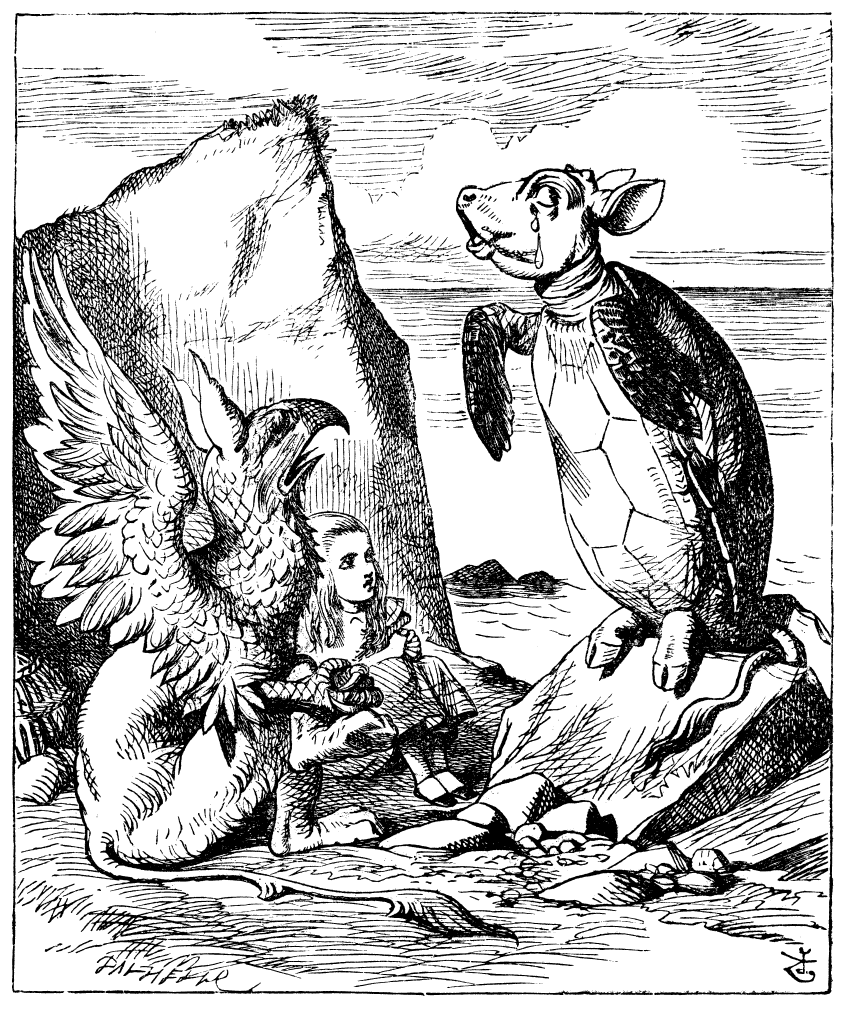
\includegraphics[height=.8\textheight]{L24/Alice_par_John_Tenniel_34.png}\\
John Tenniel's original (1865) illustration for Lewis Carroll's ``Alice in Wonderland''. Alice sitting between Gryphon and Mock turtle.
  \end{center}
\end{frame}


\begin{frame}[fragile]
  \frametitle{Mock Objects: Email Sender}
  \begin{changemargin}{1cm}
{\small
  \begin{lstlisting}
  // state or behaviour verification?
  public class MailServiceStub
                 implements MailService {
    private List<Message> messages =
        new ArrayList<Message>();
    
    public void send (Message msg) {
      messages.add(msg);
    }
    public int numberSent() {
      return messages.size();
    }
  }     
\end{lstlisting}
}
  \end{changemargin}
\end{frame}

\begin{frame}[fragile]
  \frametitle{Mock Objects: Behaviour Verification}
  \begin{changemargin}{1cm}
{\small
  \begin{lstlisting}
// jMock syntax
class OrderInteractionTester... {
  public void testOrderSendsMailIfUnfilled() {
    Order order = new Order(TALISKER, 51);
    Mock warehouse = mock(Warehouse.class); // (1)
    Mock mailer = mock(MailService.class);
    order.setMailer((MailService) mailer.proxy());

    mailer.expects(once()).method("send"); // (2)
    warehouse.expects(once()).method("hasInventory")
      .withAnyArguments()
      .will(returnValue(false));

    order.fill((Warehouse) warehouse.proxy());
  }
}    
\end{lstlisting}
}
  \end{changemargin}
\end{frame}

\begin{frame}[fragile]
  \frametitle{Mock Objects: Document Management}
  \begin{changemargin}{1cm}
{\small
  \begin{lstlisting}
// EasyMock syntax
@RunWith(EasyMockRunner.class)
public class ExampleTest {
  @TestSubject
  private ClassUnderTest classUnderTest =
      new ClassUnderTest();

  @Mock // creates a mock object
  private Collaborator mock;

  @Test
  public void testRemoveNonExistingDocument() {
    replay(mock);
    classUnderTest.removeDocument
        ("Does not exist");
  }
} 
\end{lstlisting}
}
  \end{changemargin}
\end{frame}

\begin{frame}[fragile]
  \frametitle{Mock Objects: Using a Mock}
  \begin{changemargin}{1cm}
{\small
  \begin{lstlisting}
@Test
public void testAddDocument() {
  // ** recording phase **
  // expect document addition
  mock.documentAdded("Document");
  // expect to be asked to vote for document removal, and vote for it
  expect(mock.voteForRemoval("Document"))
             .andReturn((byte) 42);
  // expect document removal
  mock.documentRemoved("Document");
  replay(mock);
  // ** replaying phase ** we expect the recorded actions to happen
  classUnderTest.addDocument("New Document",
      new byte[0]);
  // check that the behaviour actually happened:
  verify(mock);
  \end{lstlisting}
}
  \end{changemargin}
\end{frame}

\begin{frame}
  \frametitle{Flakiness: Good for croissants\footnote{thanks Pixabay}, bad for tests}
  
\includegraphics[width=\textwidth]{L24/croissant-410322_1920.jpg}
\end{frame}


\end{document}
